\documentclass[varwidth=true, border=2pt]{standalone}

\usepackage{pgfplots}
\usepackage{tikz}

\usetikzlibrary{calc,patterns,angles,quotes}

\begin{document}

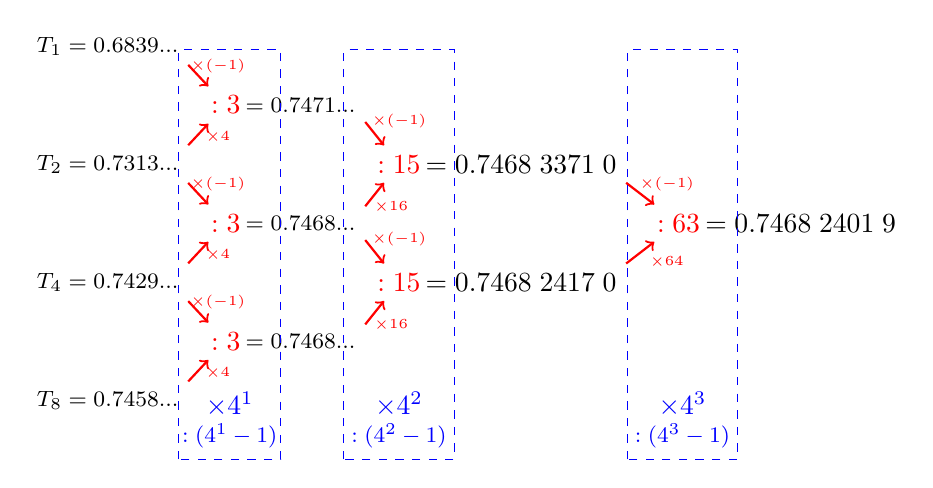
\begin{tikzpicture}


	\node (T1) at (1,5.25) {\footnotesize{$T_1 = 0.6839...$}};
	\node (T2) at (1,3.75) {\footnotesize{$T_2 = 0.7313...$}};
	\node (T4) at (1,2.25) {\footnotesize{$T_4 = 0.7429...$}};
	\node (T8) at (1,.75) {\footnotesize{$T_8 = 0.7458...$}}; %Some uncertainty about last 2 digits.  Maybe recalculate in MATLAB
	\node (A1)[red] at (2.5, 4.5){$:3$};
	\node (A2)[red] at (2.5, 3){$:3$};
	\node (A3)[red] at (2.5, 1.5){$:3$};
	
	\node (B1)at (3.45,4.5){\footnotesize{$= 0.7471...$}};
	\node (B2) at (3.45,3){\footnotesize{$= 0.7468...$}};
	\node (B3) at (3.45,1.5){\footnotesize{$= 0.7468...$}};
	\node (D1)[red] at (4.7, 3.75){$:15$};
	\node (D2)[red] at (4.7, 2.25){$:15$};
	
	\node (E1) at (6.25,3.75){$= 0.7468\;3371\;0$};
	\node (E2) at (6.25,2.25){$= 0.7468\;2417\;0$};
	
	\node (F1)[red] at (8.25, 3){$:63$};
	\node (G1) at (9.8,3){$= 0.7468\;2401\;9$};

	\draw [->, thick,red] (T1.south east) to (A1);
	\draw [->, thick,red] (T2.north east) to (A1);
	\draw [->, thick,red] (T2.south east) to (A2);
	\draw [->, thick,red] (T4.north east) to (A2);
	\draw [->, thick,red] (T4.south east) to (A3);
	\draw [->, thick,red] (T8.north east) to (A3);

	\draw [->, thick,red] (B1.south east) to (D1);
	\draw [->, thick,red] (B2.north east) to (D1);
	\draw [->, thick,red] (B2.south east) to (D2);
	\draw [->, thick,red] (B3.north east) to (D2);
	\draw [->, thick,red] (E1.south east) to (F1);
	\draw [->, thick,red] (E2.north east) to (F1);
	
	\draw[draw=blue, dashed] (1.9,0) rectangle ++(1.3,5.2);
	\draw[draw=blue, dashed] (4,0) rectangle ++(1.4,5.2);
	\draw[draw=blue, dashed] (7.6,0) rectangle ++(1.4,5.2);
	
	\node (A1a)[red] at (2.4,5){\tiny{$\times (-1)$}};
	\node (A1b)[red] at (2.4,4.1){\tiny{$\times 4$}};
	\node (A2a)[red] at (2.4,3.5){\tiny{$\times (-1)$}};	
	\node (A2b)[red] at (2.4,2.6){\tiny{$\times 4$}};
	\node (A3a)[red] at (2.4,2){\tiny{$\times (-1)$}};	
	\node (A3b)[red] at (2.4,1.1){\tiny{$\times 4$}};

	\node (D1a)[red] at (4.7,4.3){\tiny{$\times (-1)$}};
	\node (D1b)[red] at (4.6,3.2){\tiny{$\times 16$}};
	\node (D2a)[red] at (4.7,2.8){\tiny{$\times (-1)$}};
	\node (D2b)[red] at (4.6,1.7){\tiny{$\times 16$}};
	\node (F1a)[red] at (8.1,3.5){\tiny{$\times (-1)$}};
	\node (F1b)[red] at (8.1,2.5){\tiny{$\times 64$}};
	
	\node (H1a)[blue] at (2.55,0.7){$\times 4^1$};
	\node (H2a)[blue] at (4.7,0.7){$\times 4^2$};
	\node (H3a)[blue] at (8.3,0.7){$\times 4^3$};

	\node (H1b)[blue] at (2.55,0.3){\footnotesize{$:(4^1-1)$}};
	\node (H2b)[blue] at (4.7,0.3){\footnotesize{$:(4^2-1)$}};
	\node (H3b)[blue] at (8.3,0.3){\footnotesize{$:(4^3-1)$}};
	
\normalsize
	

	
\end{tikzpicture}
\end{document}